\chapter{Einleitung}

\section{Motivation und Problemstellung}

Stichpunkte:
-	Wandel von Pipeline zu Plattform-basierten Geschäftsmodellen

-	Ein sehr bekanntes Beispiel für Plattformbasierte Geschäftsmodelle sind D.Ö..

-	Neu entstehende Kundenerwartungen können nur noch erfüllt werden indem verschiedene U. zusammenarbeiten gelang es  ökosystem¬basierten  Unternehmen,  ihren  Marktwert  signifikant  zu  steigern.  Während  vor  zehn  Jahren Mineralölkonzerne und Konsumgüterfirmen das Ran¬king  der  weltweit  größten  Firmen  nach  Marktkapitalisierung  dominierten,  stehen  heute  Technologiegiganten  wie  Apple,  Amazon,  Alphabet,  Microsoft,  Tencent  oder  Alibaba  an  der  Spitze.

-	Bis 2030 werden digitale Ökosysteme weltweit einen Umsatz von rund 60 Billionen Euro erwirtschaften, und die Hoffnungen, die mit ihnen verbunden sind, sind so groß wie ihr Potenzial. (McKinsey)

-	KPMG Studie: Kompositgeschäft in der Versicherungsindustrie: Internetbasierte Ökosysteme werden nur 10 bis 15 Prozent des Marktes ausmachen, aber 30\% des Gewinns nehmen bis 2030

-	6 der 7 größten Unternehmen der Welt setzen auf digitale Ökosysteme

-	Bekanntes sehr erfolgreiches Beispiel aus Versicherungsindustrie ist der chinesische Versicherer Ping An,

-	Aus einem Anbieter von Lebensversicherungen hat sich hier ein Ökosystem entwickelt, das weit über das Kerngeschäft hinaus zu Gesundheit, Banking, Wohnen, Smart Home, Mobilität und Unterhaltung anbietet. In China umfasst eine Online-Gebrauchtwagenplattform beispielsweise integrierte Finanzdienstleistungen von Ping An Insurance. Personen, die ein gebrauchtes Auto online kaufen oder handeln, haben die Möglichkeit, am Kaufort eine Kfz-Versicherung abzuschließen - und die Kunden reagieren. Über 20\% der aktuellen Autoversicherungsverkäufe von Ping An werden derzeit über diese hochvolumige Plattform generiert.

-	Nach einer Accenture Studie ist der vielversprechende Bereich für D.Ö. in der Vers.branche der Mobility Bereich

-	Digitale Plattform bilden die technische Grundlage digitaler Ökosysteme

-	Darüber hinaus ist der Kfz-Bereich, der digitalisierteste Bereich der Branche --> Im Markt der Schaden- und Unfallversicherungen liegt der Anteil der direkt abgeschlossenen Policen hingegen bei 15,0\%. Hauptgrund dafür ist der hohe Anteil der Kfz-Versicherungen, die über Aggregatoren und die Online-Vertriebswege der Versicherer verkauft werden.










\newpage
\section{Zielsetzung und Abgrenzung}

Zielsetzung:

-	Übergeordnete Forschungsfrage: Welches Potential können Kfz-Versicherer aus digitalen Plattformen heben? --> brauch man eine Übergeordnete Frage überhaupt, kann ich diese nicht ggf. auch einfach komplettweglassen
%Wie kann die SAP Business Technology Plattform Kfz-Versicherern bei Aufbau oder Partizipation an Digitalen Ökosystemen helfen? 

-	Unterfrage 1: Welche Anforderungen muss eine technologische Plattform erfüllen, um für Kfz-Versicherer einen Mehrwert schaffen zu können?

-	Unterfrage 2: Inwiefern werden diese Anforderungen von der SAP Business Technology Plattform erfüllt?


Abgrenzung:

-	Konzentration auf den deutschen Markt

-	Begrenzung auf Erstversicherer bzw. Kfz-Versicherer, da hier das Thema D. Ö. am vielversprechendsten ist

-	Nicht im Fokus der Arbeit ist die Frage, ob Kfz-Versicherer zukünftig bei Mobilitätssystemen Orchestrator oder Teilnehmer sein werden(Ausblick)


\newpage
\section{Aufbau der Arbeit}

\begin{figure}[h]
    \centering
    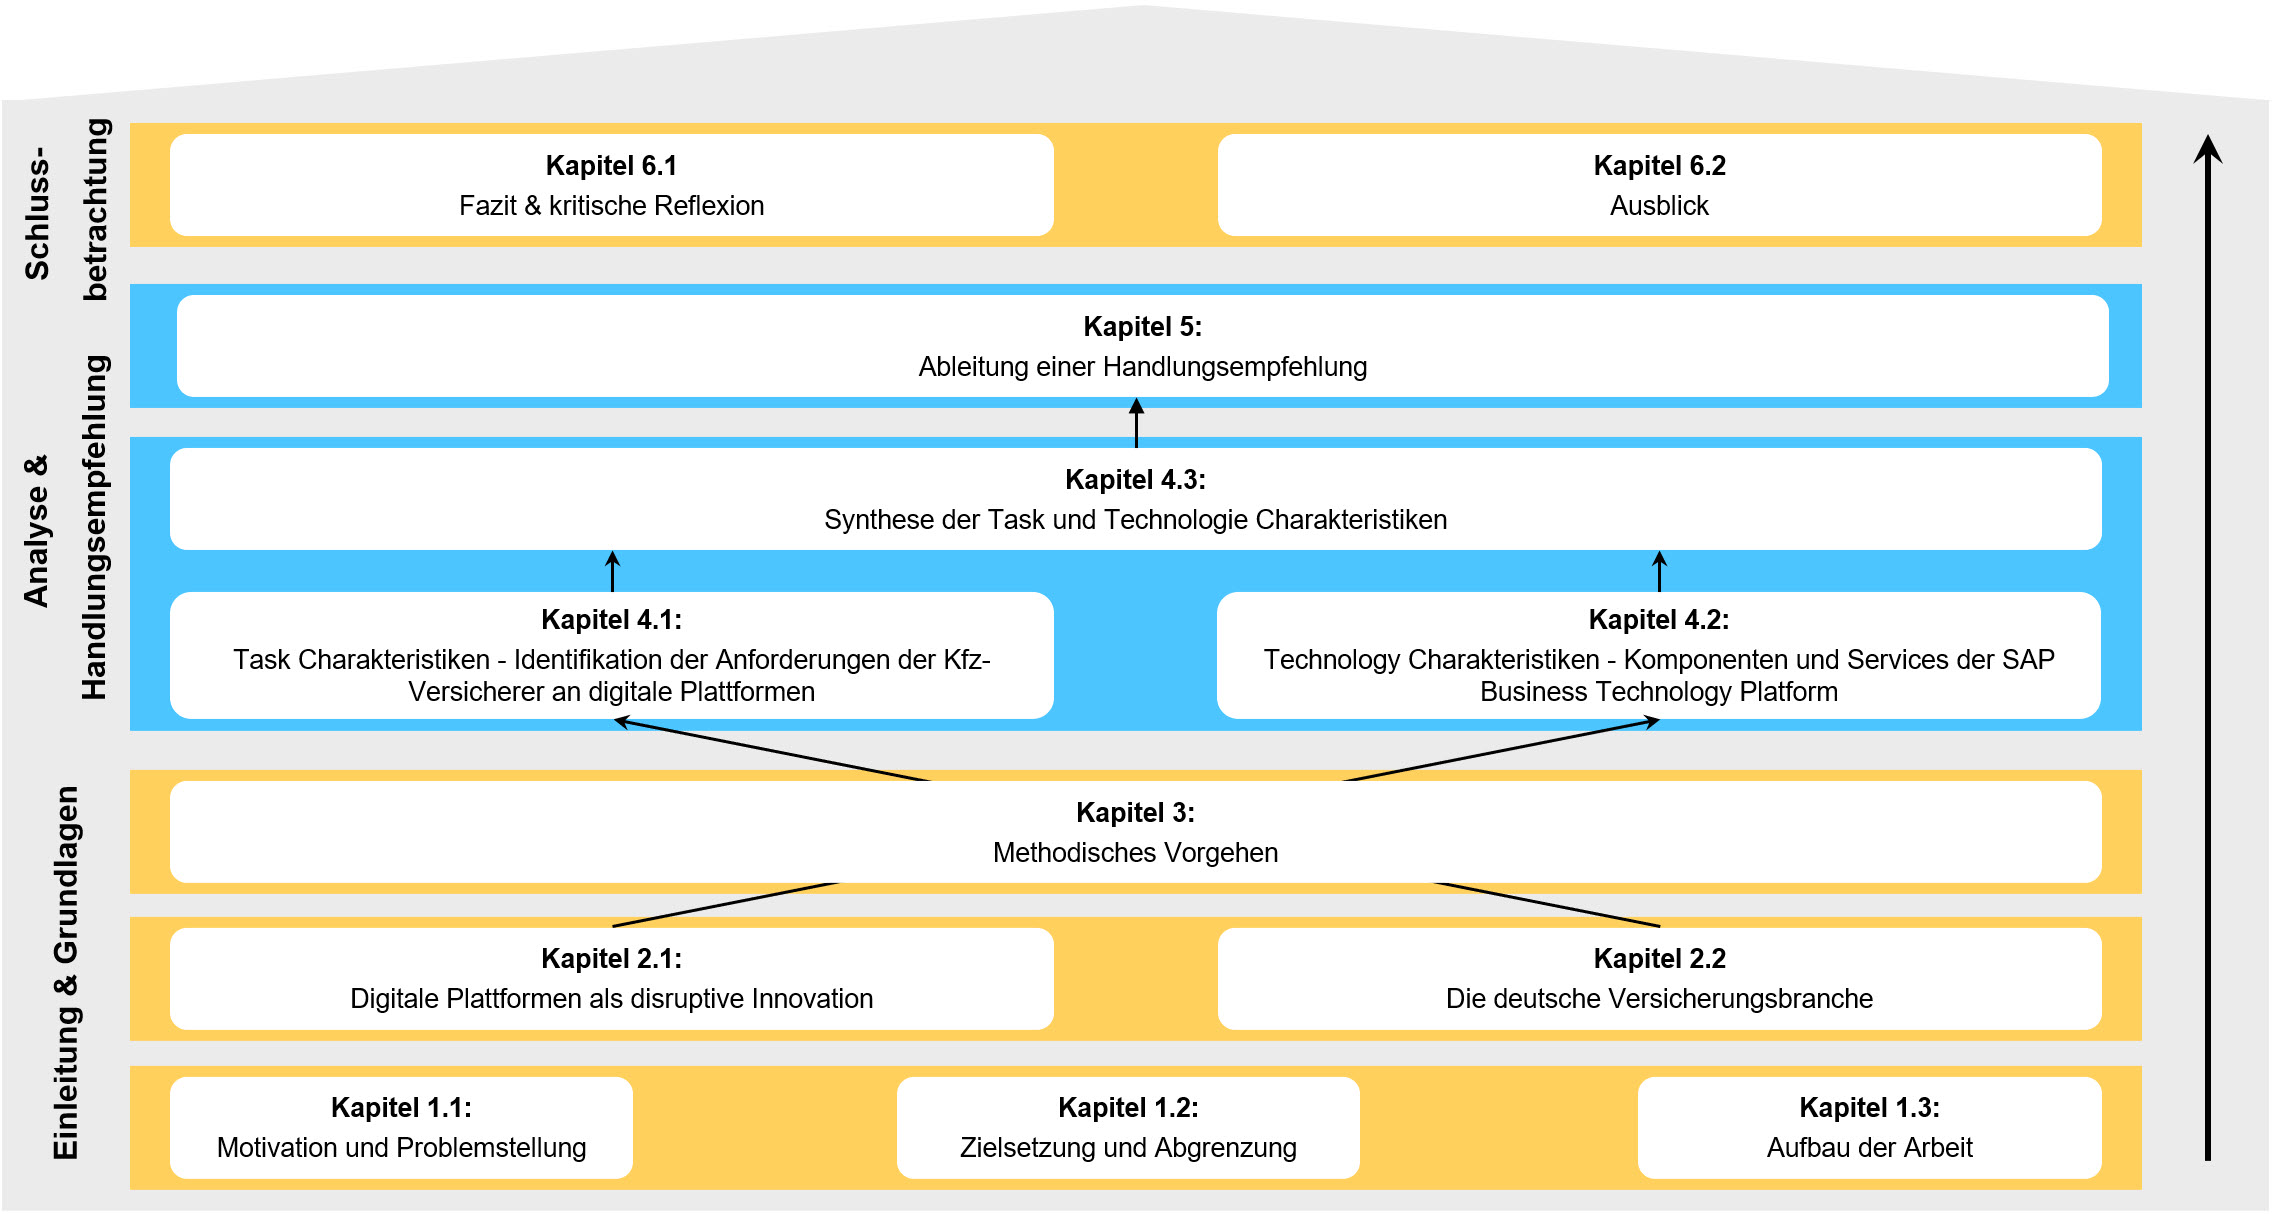
\includegraphics[width=1\textwidth]{img/Aufbau_der_Arbeit.jpg}
    \caption[Aufbau der Arbeit]{Aufbau der Arbeit\autocite{Aufbau}}
    \label{fig:Aufbau}
\end{figure}
\footnotetext{eigene Darstellung}

\newpage